% !TEX TS-program = pdflatex
% !TEX encoding = UTF-8 Unicode

% This is a simple template for a LaTeX document using the "article" class.
% See "book", "report", "letter" for other types of document.

\documentclass[11pt]{article} % use larger type; default would be 10pt

\usepackage[utf8]{inputenc} % set input encoding (not needed with XeLaTeX)

%%% Examples of Article customizations
% These packages are optional, depending whether you want the features they provide.
% See the LaTeX Companion or other references for full information.

%%% PAGE DIMENSIONS
\usepackage{geometry} % to change the page dimensions
\geometry{a4paper} % or letterpaper (US) or a5paper or....
% \geometry{margin=2in} % for example, change the margins to 2 inches all round
% \geometry{landscape} % set up the page for landscape
%   read geometry.pdf for detailed page layout information

\usepackage{graphicx} % support the \includegraphics command and options

% \usepackage[parfill]{parskip} % Activate to begin paragraphs with an empty line rather than an indent

%%% PACKAGES
\usepackage{booktabs} % for much better looking tables
\usepackage{array} % for better arrays (eg matrices) in maths
\usepackage{paralist} % very flexible & customisable lists (eg. enumerate/itemize, etc.)
\usepackage{verbatim} % adds environment for commenting out blocks of text & for better verbatim
\usepackage{subfig} % make it possible to include more than one captioned figure/table in a single float
% These packages are all incorporated in the memoir class to one degree or another...

%%% HEADERS & FOOTERS
\usepackage{fancyhdr} % This should be set AFTER setting up the page geometry
\pagestyle{fancy} % options: empty , plain , fancy
\renewcommand{\headrulewidth}{0pt} % customise the layout...
\lhead{}\chead{}\rhead{}
\lfoot{}\cfoot{\thepage}\rfoot{}

%%% SECTION TITLE APPEARANCE
\usepackage{sectsty}
\allsectionsfont{\sffamily\mdseries\upshape} % (See the fntguide.pdf for font help)
% (This matches ConTeXt defaults)

%%% ToC (table of contents) APPEARANCE
\usepackage[nottoc,notlof,notlot]{tocbibind} % Put the bibliography in the ToC
\usepackage[titles,subfigure]{tocloft} % Alter the style of the Table of Contents
\renewcommand{\cftsecfont}{\rmfamily\mdseries\upshape}
\renewcommand{\cftsecpagefont}{\rmfamily\mdseries\upshape} % No bold!

\usepackage[colorlinks,linkcolor=red]{hyperref}


%%% END Article customizations

%%% The "real" document content comes below...

\title{HW3 Report}
\author{Gong Lixue}
%\date{} % Activate to display a given date or no date (if empty),
         % otherwise the current date is printed 

\begin{document}
\maketitle

\section{Neural Networks}

The implementation of feedforward and backpropagation process is shown in code folder.
At the end of training iterations, $ loss = 1.717e-01 $, $ accuracy = 0.9400 $, which is not the optimal actually.
And for testing, $ loss = 2.522e-01 $, and $accuracy=0.9230$.

\section{K-Neareast Neighbor}
(a) boundary figures is shown below:

\begin{figure}[h]
\centering
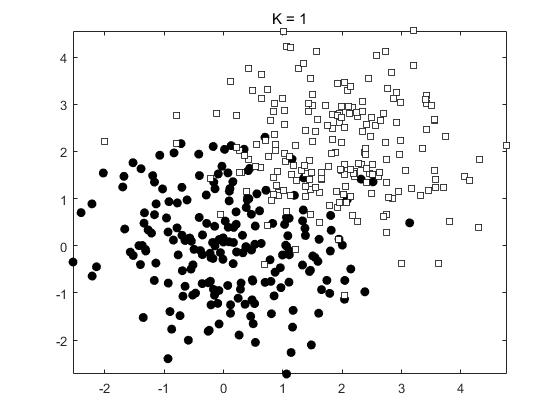
\includegraphics[width=2in]{knn_k1.jpg}  %图片名
\caption{K = 1}
\label{fig1}
\end{figure}

\begin{figure}[h]
\centering
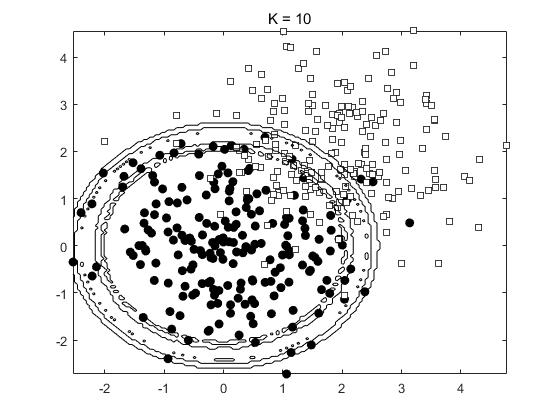
\includegraphics[width=2in]{knn_k10.jpg}  %图片名
\caption{K = 10}
\label{fig2}
\end{figure}

\begin{figure}[h]
\centering
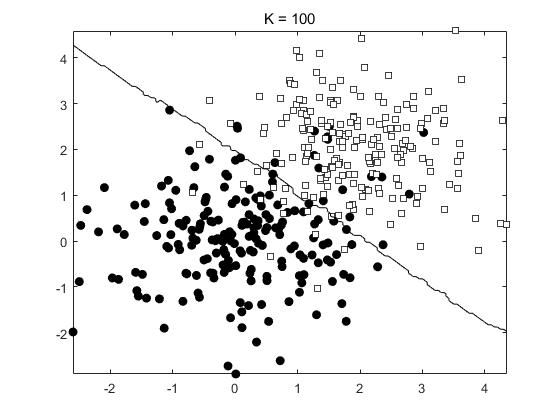
\includegraphics[width=2in]{knn_k100.jpg}  %图片名
\caption{K = 100}
\label{fig3}
\end{figure}

(b) 
One of methods is that choosing a proper K by Cross-Validation. Compute the validation error on validation set using different values for K. And pick the optimal K with the lowest validation error.

(c)
Firstly, I wrote a simple python script to fetch and save check code images from this \href{http://jwbinfosys.zju.edu.cn/default2.aspx}{website} automatically.(See Figure 4)

\begin{figure}
\centering
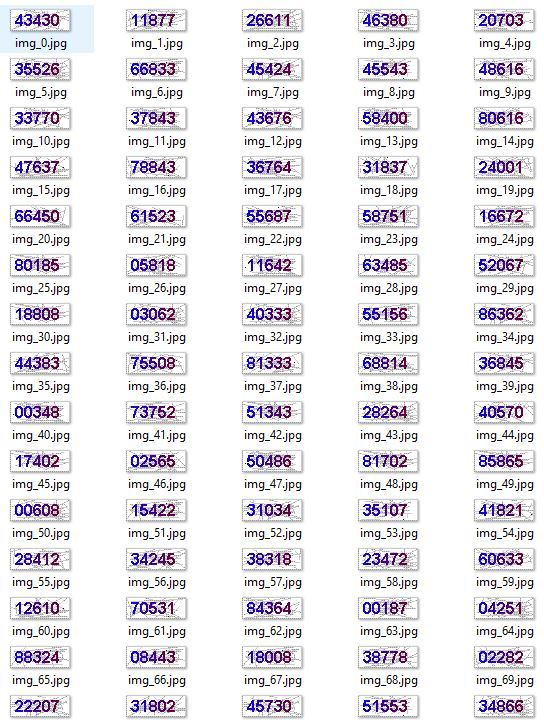
\includegraphics[height=3in]{knn_spider.jpg}  %图片名
\caption{images fetched by python spider}
\label{fig4}
\end{figure}

And then, label these images by hand. I use 100 images of them. The raw labels are recored in file  $./knn/hack_py/label\_100img.txt$. Each row in this file means the actual codes that corresponding image represents.

Before recognizing a check code image, we should generate a $.mat$ file which is used for training in knn. Run $gen\_hack\_data.m$ to generate a .mat file.
Finally, we can test the algorithm to recognize a check code image(see $knn\_exp.m$ Part2).

\begin{figure}
\centering
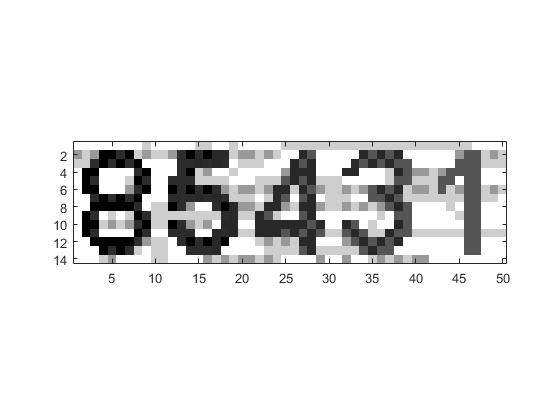
\includegraphics[width=2in]{knn_showimg.jpg}  %图片名
\caption{show\_image}
\label{fig5}
\end{figure}

\begin{figure}
\centering
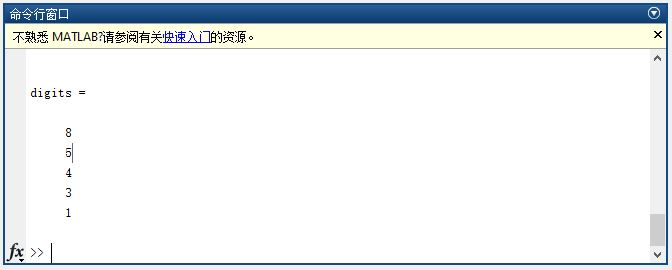
\includegraphics[width=2in]{knn_resultdigits.jpg}  %图片名
\caption{result digits}
\label{fig6}
\end{figure}


\section{Decision Tree and ID3}
The decision tree and respective information gain is illustrated as the graph below:

\begin{figure}[h]
\centering
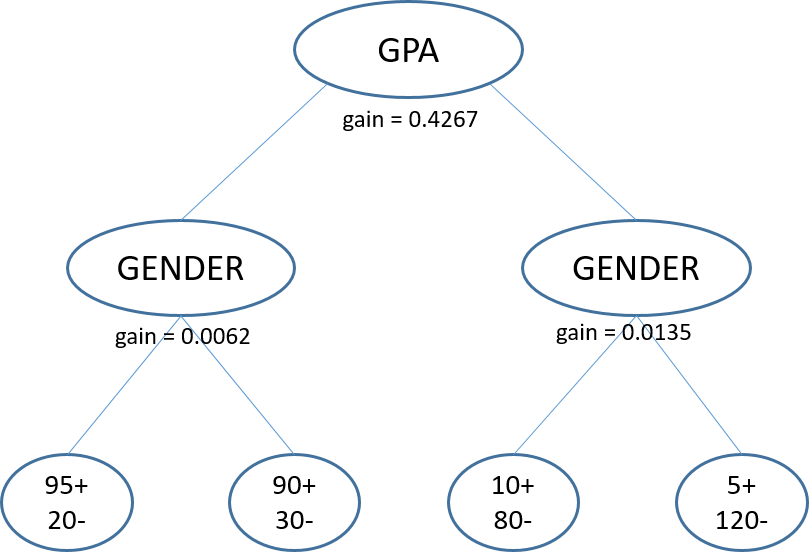
\includegraphics[width=2in]{tree.png}  %图片名
\caption{decision tree}
\label{fig4}
\end{figure}

\section{K-Means Clustering}






\end{document}




